\chapter{Normalising the Untyped Lambda Calculus}
\label{chap:untypednbe}

\section{Overview of the NbE algorithm}

\begin{figure}[h]
    \centering
    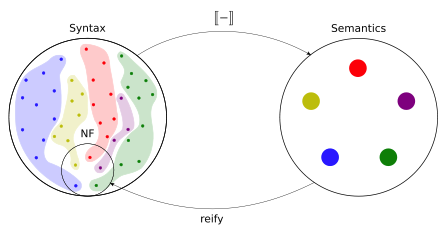
\includegraphics[width=0.7\textwidth]{./images/nbe_diagram}
    \caption{A visual overview of the NbE algorithm from \cite{slides}}
    \label{fig:nbeOverview}
\end{figure}

NbE proceeds in two steps. The first is to evaluate terms of the lambda calculus into a semantic set. In \ref{fig:nbeOverview} terms are represented by dots in the syntax set and the evaluation function is denoted by $\llbracket - \rrbracket$, which we refer to as \code{eval}. The second step is to \code{reify} the semantic value back into the normal form of the original term. Thus, the composition of \code{eval} and \code{reify} yields the \code{normalise} function which maps terms to their normal forms. 

% property of eval
\ref{fig:nbeOverview} illustrates why NbE works. The key property of the \code{eval} function is that $\beta$-equal terms (represented by dots of the same colour in the syntax set) evaluate to the same semantic value. This ensures that $\beta$-equal terms normalise to the same normal form. The key property of the \code{reify} function is that the codomain of \code{reify} is the subset of normal forms, so \code{normalise} is guaranteed to return a normal form. 

The remainder of this chapter defines the data NbE operates on and functions to perform NbE in Haskell.

\section{Gensym NbE}

\subsection{Syntax}

\begin{lstlisting}
    type Name = String

    data Expr = ExpVar Name
              | ExpLam Name Expr
              | ExpApp Expr Expr
\end{lstlisting}

Inhabitants of the inductively-defined datatype \code{Expr} are well-formed terms of the untyped lambda calculus with strings as variables. The first argument of the lambda case introduces a new variable name bound in the function body defined by the second argument. For example, the identity function $\lambda x . x$ would be encoded as \code{ExpLam "x" (ExpVar "x")}.

\begin{lstlisting}
    data NormalForm = NfNeutralForm NeutralForm
                    | NfLam Name NormalForm

    data NeutralForm = NeVar Name
                     | NeApp NeutralForm NormalForm
\end{lstlisting}

We now define the target syntax of the \code{normalise} function, \code{NormalForm}. Note that \code{NormalForm} is inhabited by all the terms not containing $\beta$-redexes \cite{slides}, since the definition of \code{NeApp} only permits application on non-lambda terms, which are encoded as values of type \code{NeutralForm}.

\subsection{Semantics}

\begin{lstlisting}
    data V = Neutral NeutralV
           | Function (V -> V)

    data NeutralV = NeVVar Name
                  | NeVApp NeutralV V
\end{lstlisting}

% TODO: Mentional easy to define V -> V in Haskell, harder in other languages, motivating advantage of Haskell?

The semantic set \code{V} has a very similar structure to the set of normal forms, however lambda terms are replaced with Haskell functions of type \code{V} $\rightarrow$ \code{V}.
% TODO: Include following paragraph or not - not justified? 
The similarity simplifies \code{reify} as for some terms there are obvious translations from semantics to syntax. The replacement of lambda terms will be useful in evaluating $\beta$-redexes at the semantic level instead of the syntactic level. 

% TODO: Discuss using why don't use Neutral Form but establish our own datatype

\subsection{Evaluation}

Evaluation proceeds by pattern matching on the given term, and evaluating its constituent subterms. However, the semantic meaning of subterms can differ depending on which variables are bound by which lambda term. For example, in the terms $\lambda x . \lambda y . xy$ and $\lambda y . xy$, the semantic meaning of the $xy$ subterm is different. Thus, in addition to the term itself, \code{eval} needs information about the bound variables introduced by surrounding lambda terms. 

To keep track of which variables have been bound by surrounding lambda terms, we construct an environment datatype.

\begin{lstlisting}
    type Env = Map Name V
\end{lstlisting}

Each key of the map corresponds to a bound variable name, and its associated value is the semantic value representing the variable. The environment can be thought of as the scope each subterm is evaluated in. 
% TODO: Include or not - helpful or overly general waffle?
It expands as more variables are bound in deeper subterms.

\begin{lstlisting}
    eval :: Expr -> Env -> V
\end{lstlisting}

\code{eval} takes an expression and the environment to evaluate it in, pattern matches on the expression, and returns the interpretation of the term in the semantic set. We now discuss the implementation of each case of the pattern match.

\begin{lstlisting}
    eval (ExpVar x) env = case lookup x env of
        Just y -> y
        Nothing -> Neutral (NeVVar x)
\end{lstlisting}

In the variable case, we lookup the variable in the environment. If the variable was bound by a surrounding lambda term, the variable will be present in the environment, and we can return the semantic value associated with it. Otherwise, the variables is free, so we return a semantic variable with the same name.

\begin{lstlisting}
    eval (ExpLam var m) env = Function f where
        f :: V -> V
        f v = eval m env' where
            env' = insert var v env
\end{lstlisting}

% TODO: Include or not, repeating code in words?
The semantic interpretation of a lambda expression is a Haskell function of type \code{V} $\rightarrow$ \code{V}. This function takes an element \code{v} of the semantic set \code{V}, and returns the body of the lambda evaluated in an extended environment \code{env'}. In this extended environment, we bind the named variable \code{var} to \code{v}.

From the variable case, we see that whenever the variable \code{ExpVar var} is evaluated in the function body it will be interpreted as \code{v}. We can think of \code{v} as a semantic placeholder for the value \code{f} is applied to (if any). The use of this approach is demonstrated in the application case.

\begin{lstlisting}
    eval (ExpApp m n) env = app (eval m env) (eval n env)
        where
            app :: V -> V -> V
            app (Function f) v0 = f v0
            app (Neutral n)  v0 = Neutral (NeVApp n v0)
\end{lstlisting}

In the application case we evaluate the \code{m} and \code{n} terms in the same environment, before applying them to \code{app}, which handles the application of semantic values. 

In the case where the first value is a function \code{f}, we evaluate \code{f} at the second argument \code{v0}. From the lambda case we see that this subcase corresponds to evaluating a redex term. Instead of contracting the redex by substituting at the syntactic level, we evaluate it using function application at the semantic level. The application instantiates the placeholder \code{v} at the semantic value \code{v0} in the lambda body. 

% TODO: Explain more
In the case that the first value is a value \code{n} of type \code{NeutralV}, there is no redex to contract, so we return a placeholder Neutral application at the semantic level.

\subsection{Reification}

% TODO: Cite name, in de Bruijn paper

Reification proceeds by pattern matching on the semantic value, and recursively reifying its constituent values.

Since evaluating a lambda yields a function, reifying a function should yield a lambda to ensure that \code{normalise} preserves terms already in normal form. But what variable should the returned lambda term bind? The new bound variable should be different to all other bound variables in scope, otherwise \code{reify} could produce invalid terms. It should also be different to all other free variables in the original term, to prevent free variable capture. Since terms are considered equal up to bound variable renaming by $\alpha$-equivalence, we can choose any variable name that satisfies these requirements. 

One approach to resolve this issue suggested by \cite{slides} is to generate a fresh variable name during reification whenever a new bound variable is needed. However, generating fresh variables during the execution of \code{reify} would require the function to track which variables have already been bound between calls to \code{reify}, which suggests the use of state. This could be modelled using the \code{State} monad, in which case \code{reify} would have the type signature \code{reify :: V -> State [Name] NormalForm}, where \code{[Name]} corresponds to a list of variable names that have already been bound. This would allow us to implicitly pass the list of bound variable names between calls to reify. However state introduces additional complexity and makes testing more difficult, which can lead to flawed implementations.

%TODO: other problems with state monad (not really used mostly passing => redundant boilderplate to carry monad round), link to State monad implementation

Instead, we opt for a more functional approach. Before the execution of \code{reify}, we generate a suitable stream of fresh variable names of type \code{[Name]}. By making \code{reify} a function of the semantic element and the stream of fresh variables, we can simply pop a fresh variable name from the stream whenever a new variable is bound. In recursive calls, \code{reify} only passes the tail of the stream to ensure bound variable names are never reused.

\begin{lstlisting}
    reify :: V -> [Name] -> NormalForm
\end{lstlisting}

\code{reify} proceeds by pattern matching on the first argument of type \code{V}. 

\begin{lstlisting}
    reify (Neutral n)  freshVars = NfNeutralForm (reifyNeutral n freshVars)
        where
            reifyNeutral :: NeutralV -> [Name] -> NeutralForm
            reifyNeutral (NeVVar i)   freshVars = NeVar i
            reifyNeutral (NeVApp n m) freshVars = NeApp reifiedN reifiedM
                where
                    reifiedN = reifyNeutral n freshVars
                    reifiedM = reify m freshVars
\end{lstlisting}

In the neutral case, we use \code{reifyNeutral} to convert the value \code{n} of type \code{NeutralV} to a \code{NeutralForm}, which is promoted to a \code{NormalForm} by the \code{NfNeutralForm} constructor. The \code{reifyNeutral} function also proceeds by patten matching. 

In the variable case we extract a neutral syntactic variable of the same name as the semantic variable. 

In the application case we reify the semantic values \code{n} and \code{m}, and return a neutral syntactic application of the resulting terms.
% TODO: Check this - talk about independece between reifyiedN and reifiedM, reword
We are able to reify both semantic values using the same fresh variable stream since the returned value is a \code{NeutralForm}, which by definition contains no redexes. This means \code{reifiedM} will not be substituted into \code{reifiedN}, so there will not be any variable name clashes.
For example, in the neutral term $(y(\lambda x.x))(\lambda x . x)$ there is no issue in the left and right terms reusing $x$ as a bound variable since there is no ambiguity about which $x$ is being referred to in any part of the term. Since there are no redexes to contract, there is no need to rename the bound variables.

% TODO: Define 'original term', 'surrounding lambdas'

\begin{lstlisting}
    reify (Function f) (v:vs)   = NfLam v body
    where 
        body = reify (f (Neutral (NeVVar v))) vs
\end{lstlisting}

The reification of an abstract semantic function \code{f} produces a concrete syntactic description for \code{f}. \code{reify} abstracts out the argument of \code{f} into a syntactic variable \code{v} with a lambda expression. In the body of \code{f}, we replace the abstract argument with the variable \code{v} by applying \code{f} to \code{Neutral (NeVVar v)}. This value has type \code{V}, so we can \code{reify} it to produce a syntactic representation for the body of \code{f}, which completes the term. We \code{reify} the term with the stream of fresh variables \code{vs}, since the variable name \code{v} is bound in the body of the lambda, so is no longer fresh.

\subsection{Normalisation}

Using the implementations of \code{eval} and \code{reify}, we can define the \code{normalise} function as follows.

\begin{lstlisting}
    normalise :: Expr -> NormalForm
    normalise exp = reify (eval exp Map.empty) freshNames
        where
            freshNames = (getFreshVariableStream . getFreeVariables) exp
\end{lstlisting}

\code{normalise} takes an expression, and returns its normal form. Since \code{normalise} returns a value of type \code{NormalForm} it is guaranteed that the returned expression is normal. First we evaluate the given expression in the empty environment, since no variables are bound to begin with. Then we reify the returned semantic value of type \code{V} back into a concrete \code{NormalForm} term. 

Some terms such as $(\lambda x.x x)(\lambda x.x x)$ do not have a normal form. However, the \code{normalise} type signature guarantees that all expressions can be normalised to a normal form. The resolution to this paradox is that in cases where terms do not have a normal form, \code{normalise} will not terminate so will never produce a normal form. In particular, such expressions do not have a representation in the semantic state, so \code{eval} never terminates. For example, when evaluating $(\lambda x.x x)(\lambda x.x x)$, \code{eval} reaches a stage where it must evaluate the Haskell application \code{(\v -> app v v) (\v -> app v v)}. Following the definition of \code{app}, we find that this evaluates to the same expression, and thus will never finish evaluating. This is similar to the corresponding $\beta$-reduction, where $(\lambda x.x x)(\lambda x.x x) \rightarrow_\beta (\lambda x.x x)(\lambda x.x x)$, except that in NbE this infinte contraction happens in the semantics.

We produce a stream of valid fresh variable names \code{freshVars} of type \code{[Name]} for the given expression using the following functions.

\begin{lstlisting}
    getFreeVariables :: Expr -> Set Name
    getFreeVariables (ExpVar x)   = singleton x
    getFreeVariables (ExpLam x m) = delete x (getFreeVariables m)
    getFreeVariables (ExpApp m n) = getFreeVariables m `union` getFreeVariables n

    getFreshVariableStream :: Set Name -> [Name]
    getFreshVariableStream freeVars = [freshVariable i | i <- [0..], 
                                       notMember (freshVariable i) freeVars] 
        where
            freshVariable i = "v" ++ show i
\end{lstlisting}

\code{getFreeVariables} takes an expression and returns the set of free variable names. \code{getFreshVariableStream} takes the set of free variable names and returns a stream of fresh variable names, since each of the names are distinct from each other and the free variables.

\section{de Bruijn NbE}

\subsection{Motivation}

While the Gensym approach works, generating fresh variables is a fragile procedure. The correctness of \code{normalise} depends on it, however mistakes in the implementation would be easy to make and difficult to notice. Another drawback of the Gensym approach is that \code{reify} is indexed by an infinite stream of variable names, which is difficult to reason about.

One approach to resolve the fresh variable problem is to remove variable names from the syntax altogether, by using an alternative representation of lambda calculus terms. In general, a variable can be thought of as a pointer to the lambda that binds it. Named terms do this by labelling lambdas and referencing them in variables using their names. de Bruijn terms take a different approach which we describe below, but fundamentally both approaches serve the same purpose, so represent the same set of terms.

\subsection{Introduction to de Bruijn Terms}

de Bruijn terms are defined as follows. \cite{deBruijnNotation}

\begin{lstlisting}
    data DbExpr = DbVar Int
                | DbLam DbExpr
                | DbApp DbExpr DbExpr
\end{lstlisting}

In de Bruijn terms, lambda terms are not named, as seen in the definition of \code{DbLam}. Instead, each variable refers to the lambda that binds it using a de Bruijn index: the number of lambdas between the occurrence of the variable and the lambda which binds it. If we think of the set of bound variables at each point of the term as a stack, with the most recently bound variable at the top, then the de Bruijn index of a variable is the number of bindings you have to pop from the scope stack to reach the variable.

\begin{figure}[h]
    \centering
    \begin{tabular}{ |c|c| } 
        \hline
        Named Notation & de Bruijn Notation \\
        \hline 
        $\lambda x.x$ & $\lambda . 0$ \\
        $(\lambda x. x)(\lambda y . y)$ & $(\lambda . 0)(\lambda . 0)$ \\
        $\lambda x. x (\lambda y. x y)$ & $\lambda . 0 (\lambda . 1 0 )$ \\
        \hline
    \end{tabular}
    \caption{Examples of de Bruijn terms and their equivalent named terms}
    \label{fig:deBruijnExamples}
\end{figure}


% TODO: Think about dB NBE acting on standalone dB terms
% Do we need more presise valid terms
% Don't want to make assumptions about pre-processing/data format, restrictions should be encoded in program


Variables with indices greater than the number of bound lambdas are treated as free. For example, we could represent the term $y (\lambda x.xy)$ as $0 (\lambda .01)$ using de Bruijn terms. In the above term we have implicitly bound the free variable $y$ to 0 at the top level of the term. Note that we refer to $y$ using the index $1$ inside the lambda since the lambda introduces a bound variable in the context of its body. 2 $(\lambda . 0 3)$ is an equivalent term where $y$ is implicitly bound to 2 at the top level.

We now define NbE for the de Bruijn lambda calculus terms. Our implementation is inspired by an implementation by Andreas Abel \cite{deBruijn}, but diverges from it to improve type-safety.

\subsection{Syntax}

The changes to the syntax are reflected in the definition of the de Bruijn normal and neutral terms. 

\begin{lstlisting}
    data NormalForm = NfNeutralForm NeutralForm
                    | NfLam NormalForm

    data NeutralForm = NeVar Int
                     | NeApp NeutralForm NormalForm
\end{lstlisting}

\subsection{Semantics}

We also redefine the semantic set for de Bruijn terms.

\begin{lstlisting}
    data V = Neutral NeutralV
           | Function (V -> V)

    data NeutralV = NeVFreeVar Int
                  | NeVBoundVar Int
                  | NeVApp NeutralV V
\end{lstlisting}

Our implementation uses distinct constructors to distinguish between free and bound variables in the semantic set, which makes it easier to understand the operation of the code and improves type safety.

% TODO: De Bruijn levels not indicies - motivate with problem as indicies dependent on full term but want V to fully define 

\subsection{Evaluation}

\begin{lstlisting}
    type Env = Map Int V
\end{lstlisting}

In the de Bruijn implementation, the environment maps from de Bruijn indices to the semantic set, instead of from names.

The \code{eval} function for de Bruijn terms operates similarly to the gensym evaluation function

\begin{lstlisting}
    eval :: Env -> DbExpr -> V
    eval env (DbVar x) = case lookup x env of
        Just y -> y
        Nothing -> Neutral (NeVFreeVar (x - size env))
\end{lstlisting}

In the variable case we lookup the semantic interpretation of bound variables from the environment. 

% Q: Remove START
In Abel's implementation, all the free variables are bound to semantic values in the initial environment before evaluation begins. Since we assume that all variables are present in the environment, in the \code{Nothing} case of the variable lookup, we would have to return \code{undefined}. The algorithm is only correct if initial environment binds all free variables. Avoiding fragile pre-processing and implicit assumptions was the motivation for moving to de Bruijn notation, so we have modified Abel's implementation to improve type-safety.

Instead of assuming all free variables are already bound in the environment, we generate their semantic interpretations as we evaluate the term. We start with an empty initial environment, so the \code{Nothing} case corresponds to evaluation of a free variable, as it did in the named implementation. 

% Q: Remove END

de Bruijn indices are not suitable for indexing variables in the semantic set, as they are the dependent on the number of bindings in the context in which they occur. This context will change as redexes are contracted and lambda bindings removed by \code{eval}. We choose a semantic representation for free variables where all occurrences of the same free variable are identified with the same semantic value.
\code{eval} returns a semantic variable with the index of same variable at the outermost context of the term. It calculates this by subtracting the number of bindings in the current context (\code{size env}) from the syntactic index \code{x}. Thus, every occurrence of the free variable will be identified with the same semantic value, regardless of where it occurs in the term. 

\begin{lstlisting}
    eval env (DbLam m) = Function f where
    f :: V -> V
    f v = eval env' m where
        env' = insert 0 v (mapKeys (+1) env)
\end{lstlisting}

As in the named approach, the semantic representation chosen for functions is a Haskell function that takes a semantic value \code{v}, and returns the semantic interpretation of the lambda body with the bound variable interpreted as \code{v}. They key difference to the named implementation is the construction of the new environment. We first increment all other indices by 1, since we have introduced a new lambda between each variable and its associated binding. Then, to introduce the new variable bound by the lambda into the environment, we bind the 0th index to \code{v} in the shifted environment.

The application case remains exactly the same as in the Gensym implementation since the approach for contracting redexes is identical.

\subsection{Reification}

\begin{lstlisting}
    reify :: Int -> V -> NormalForm
\end{lstlisting}

Reification for de Bruijn terms also follows a similar structure to the Gensym approach. However, instead of taking a stream of fresh variables, the de Bruijn \code{reify} function only needs the number of bound variables in the semantic value of type \code{V}. This is significantly easier to reason about than the Gensym \code{reify} function.

\begin{lstlisting}
    reify n (Function f) = NfLam (reify (n + 1) (f (Neutral (NeVBoundVar n))))
\end{lstlisting}

As in the untyped implementation, to reify a function \code{f} we return a lambda where the body of the term is the reification of \code{f} at a fresh variable.

We use de Bruijn levels to represent bound variables in the semantic set, as Abel does in his implementation. de Bruijn levels work in the opposite way to indices: the de Bruijn level 0 corresponds to the oldest bound variable in scope, rather than the newest. 

Since \code{n} variables are bound in \code{f}, the de Bruijn levels which have already been bound are $0, 1, \dots, n - 1$. Thus, \code{NeVBoundVar n} is a fresh variable. Since we have introduced a new bound variable, we increment \code{n} by one when reifying the body of \code{f}.

\begin{lstlisting}
    reify n (Neutral m)  = NfNeutralForm (reifyNeutral n m)
        where
            reifyNeutral :: Int -> NeutralV -> NeutralForm
            reifyNeutral n (NeVFreeVar k)  = NeVar (n + k)
            reifyNeutral n (NeVBoundVar k) = NeVar (n - 1 - k)
            reifyNeutral n (NeVApp p q)    = NeApp (reifyNeutral n p) (reify n q)
\end{lstlisting}

Since the first \code{n} de Bruijn indices refer to bound variables, to reify a free variable, we increment the index of the variable at the outermost context of the term \code{k} by \code{n}.
To reify a bound variable, we translate the de Bruijn level \code{k} back to its corresponding de Bruijn index \code{n - 1 - k}.

\subsection{Normalisation}

\begin{lstlisting}
    normalise :: DbExpr -> NormalForm
    normalise = reify 0 . eval initialEnv where
        initialEnv = Map.empty  
\end{lstlisting}

To \code{normalise} de Bruijn expressions, we first evaluate the term in the empty environment and then reify the expression which initially has no bound variables. As in the untyped implementation, we have the same guarantees and caveats for normalisation. However, we have achieved our goal of removing the need for a fresh name stream.